\documentclass[12pt]{report}
\usepackage[margin=1in]{geometry}
\usepackage[english]{babel}
\usepackage{graphicx}

\begin{document}
\title{MSB Final Project: The Genetics of Music}
\author{Kabir Gupta}
\date{\today}
\maketitle

\chapter*{Introduction}
One of Tinbergen's four causes of behavior is development, or ontogeny: the question of how a behavior came to an organism in the first place. While this subject can delve deep into Mendellian inheritance and meiosis, or different forms of learning and different classifications of innate behaviors, the central and highest-level question asked during the study of development is that of nature versus nurture: is the trait genetically inherited or environmentally acquired? Of course, traits are often not one or the other but will rather fall on a spectrum between the two; the purpose of this project is to study one such trait in hopes of determining whether it is influenced more by genes or environment. This trait is musical taste: what kinds of music do people like to listen to?

It is surprisingly common, in the researcher's own (anecdotal) experience, to find two friends who have vastly different music tastes, and the same applies to family members. This leads into the question of who makes more of an impact on your music tastes --- friends will often attest to have virtually identical music taste, but the same could apply to family members; it only seems to vary from person to person and family to family. By gathering a large sample of data, however, it could be determined whether there is actually some sort of trend, or association, between a person's music tastes and their friends'/family's.

It was expected that both family members and friends would have a significant impact on a person's music choices, although one might not necessarily outweigh the other: that is, there may not be a significant difference between the family's impact and the friends'. This is because people have very strong reasons to like similar music to both a family member and a friend, so that one relationship type should not be significantly closer than the other.

\chapter*{Materials and Methods}
A Google Forms survey was used to gather data for this study. Each respondent was asked to select the musical genres that they enjoy out of 6 options: pop, jazz/blues, rock, country/folk, rap/hip hop, and classical. The respondent was then asked to decide whether they like or dislike each of 12 musical clips, out of which each genre was represented by two clips: Uptown Funk and Dead Girl in the Pool (pop), What a Wonderful World and The Thrill is Gone (jazz and blues), Bohemian Rhapsody and Hurt (rock), Old Town Road and I Walk the Line (country and folk), Rap God and Gangsta's Paradise (rap and hip hop), and finally Eine Kleine Nachtmusike and Duel of the Fates (classical).

I wanted to identify whether there were some genres that the respondent did not necessarily dislike, even if it was not something they thought they actively listen to. So, while the first part of the survey asked for what they thought they like, the second part of the survey was in an attempt to see what they might actually like. However, it's possible that somebody who generally likes a certain genre did not like the specific two clips that they had been asked about from that genre. So, the question about categories needed to be weighted more heavily than the questions about specific songs. Further, an overall system was needed for condensing the 2-part data that would be gathered --- genre and music preference, both on nominal scales --- into one number that could be used in statistical testing. Hence, the following scoring system was created, as seen in Figure 1.

\begin{figure}[h!]
  \centerline{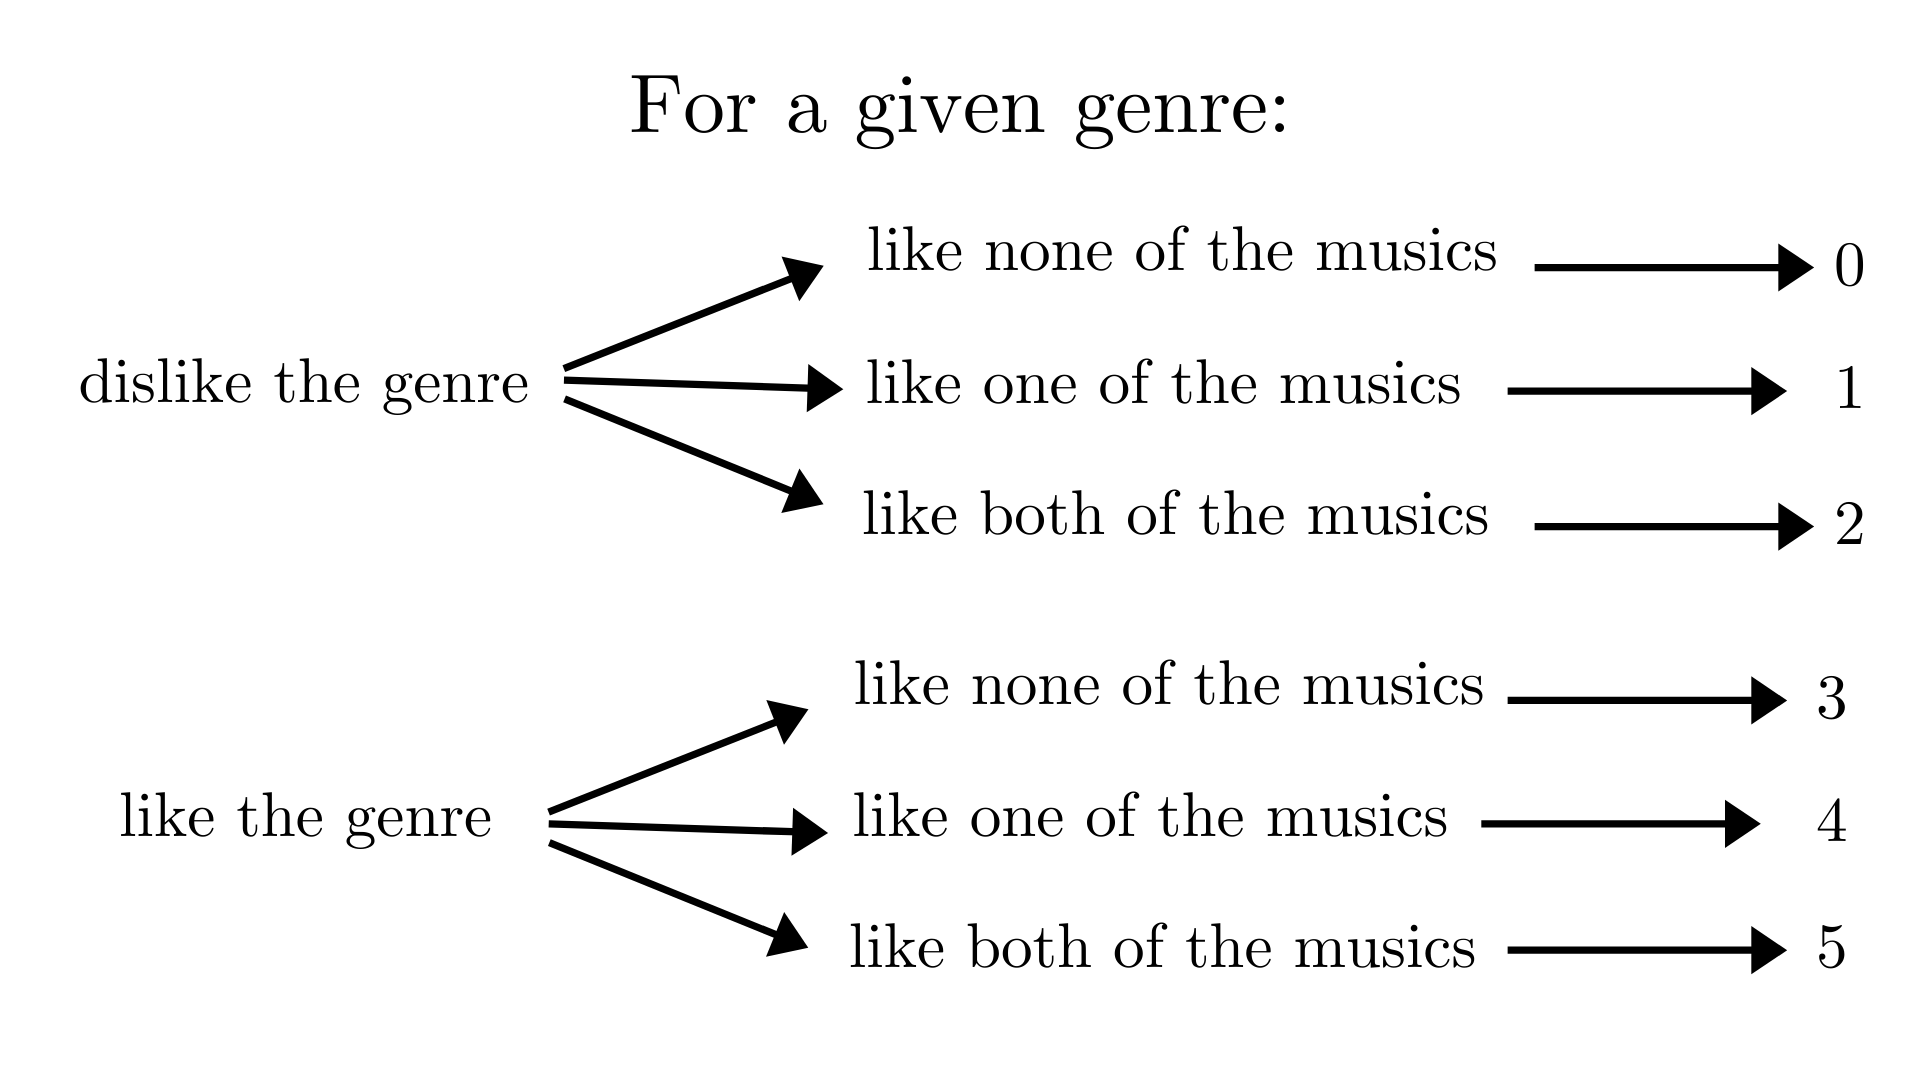
\includegraphics[width=0.5\linewidth]{matrix.png}}
  \caption{\small The procedure used to generate ordinal-scale scores for each respondent, for each genre.}
\end{figure}

This means that if a respondent says they enjoy a particular genre but doesn't like any of the musics, they can still walk away with a score of 3, whereas if they liked both musics but said they disliked the genre in general, they would only get a 2. These rankings are on an ordinal scale, from 0 to 5 (where there are no defined intervals between ranks).

Each respondent was requested to provide the names of two friends and two family members. The family members were sent a slightly different survey, which was identical to the one for students except that it did not ask them for the names of their friends or family members. At the end of data collection, each respondent was matched up to their two family members and two friends to perform statistical analysis. If not all of the family members and friends listed had responded to the survey, only the ones whose responses were present were tested against the student.

\chapter*{Data}
There were two main variables being compared in this study: relationship type (family member or friend), on a nominal (binary) scale; and genre rankings that demonstrate the degree to which someone enjoys a particular genre, on an ordinal scale.

\begin{figure}[h!]
  \centerline{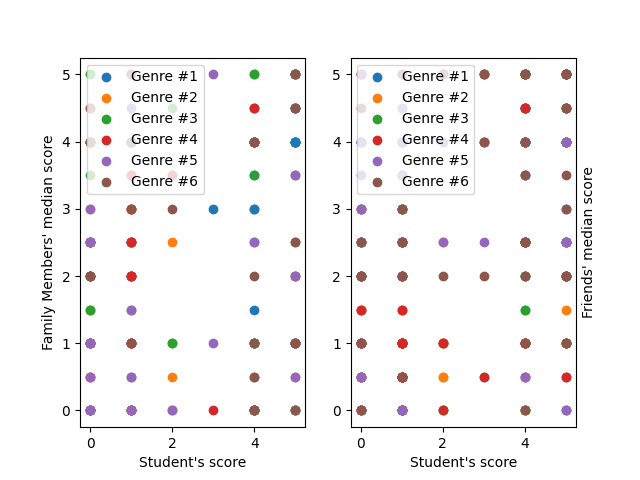
\includegraphics{scatter_plots.png}}
  \caption{\small Scatter plots displaying the data gathered. At left, each student's score is plotted against the median of their family members' scores for each genre; at right, each student's score is plotted against the median of their friends' scores for each genre.}
\end{figure}

Above (Figures 2-7), the series of bar graphs display the data gathered as relationship type by rankings for each genre. The raw data gathered during this study is included in Appendix 1/I/A.

%do i include my raw data?? it has names, do i take out the names and include it?
%what would be an appropriate form of data presentation? nom. scale is usually pie chart or bar graph but how would that work in my case??

Python Pseudocode:
    def GetListOfNames:
        list of names
        column.foreach(name)
            add name to list

    def Anonymize:
           var counter = 0
           for name in names
                name = counter
                counter += 1


\chapter*{Statistical Analysis}
%i used rankings
%then WC
%then X^2
%then SRCC but how to interpret??


\chapter*{Discussion}
%insignificant sooo

\chapter*{References}
%include the songs?? what about GForms?
%lincoln helped with code review twice already, credit them? ack and tommy now
%cite scipy and all the timestamps for the music

%might be nice to include my code, i've seen Appendices be used in studies, would that be a good idea??
1 This research was supported by a grant from Your Mom Institute. Special thanks to Dr. Your Mom and an anonymous reviewer for catching mistakes and offering helpful advice.



\end{document}
